\subsubsection{MVC-Struktur}\label{subsec:mvc}

Das MVC-Framework wird zur Softwarestrukturierung verwendet. Durch diese Strukturierung werden die Berechnungen der Daten (eng. model), die Steuerung (engl. controller) und dessen graphischer Repräsentation (engl. view) getrennt. In der Abbildung \ref{fig:MVCBeispiel} ist dieser Aufbau in einem Beispielklassendiagramm dargestellt. \cite{MVCDesignPattern}

\begin{figure}[H]
	\centering
	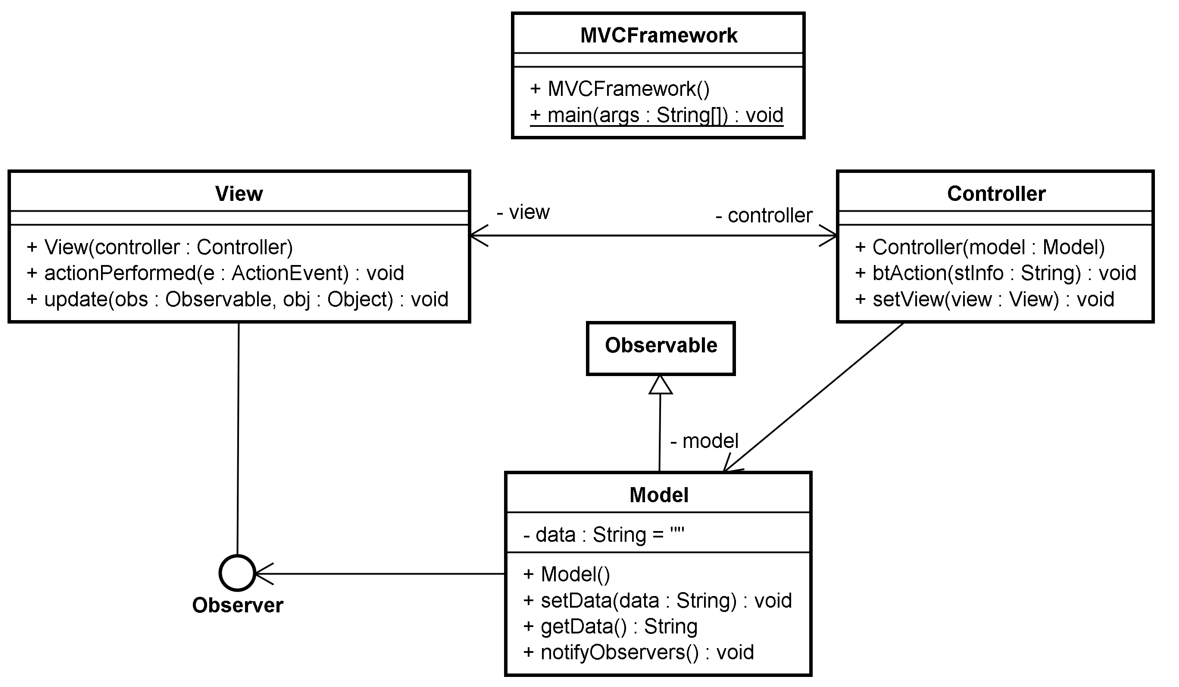
\includegraphics[width = 10cm]{MVC_Beispiel.png}
	\caption{MVC Beispielklassendiagramm \cite{MVCBeispiel}}
	\label{fig:MVCBeispiel}
\end{figure}

Der Ablauf dieser Struktur ist wie folgt: 

\begin{enumerate}
\item Benutzereingabe löst Event aus
\item Die Aktion wird dem Controller übergeben. Dieser holt die Daten in der View, leitet diese dem Model weiter und löst die Berechnungen aus
\item Das Model führt die Berechnungen aus und informiert den Observer
\item Der Observer löst ein Event in der View aus. View kann die Daten vom Model holen und ausgeben
\end{enumerate}
